\section{Evaluation}
\label{sec:evaluation}

This section has two goals. First, we want to compare our fragmentation approach to other model persistence frameworks. Secondly, we want to verify our findings from section~\ref{sec:gains}. 
All measurements were performed on a Notebook computer with Intel Core i5 2.4\.GHz CPU, 8 GB 1067 MHz DDR3 RAM, running Mac OS 10.7.3. All experiments were repeated at least 20 times, and all present results are respective averages. Code executing all measurements and all measured data can be downloaded as part of EMFFrag~\cite{EMFFragProject}.

\subsection{Fragmentation Compared to other Persistence Frameworks}

To compare fragmentation to EMF's XMI implementation, CDO, and Morsa, we measured execution time for the three tasks (i) create/modify, (ii) traverse, and (ii) query. To analyze traverse and query, we used example models from the Grabats 2009 contest~\cite{grabats} as benchmarks. Those were already used to compare Morsa with XMI and CDO here~\cite{morsa2011}. There are five example models labeled \emph{set0} to \emph{set4} and they all model Java software based on the same meta-model. Please note: even though the models increase in size, their growth is not linear and the internal model structure is different. To measure create/modify performance, we used a simple test model. We don't provide any comparative measures for partial loads. Partial loads are extensively measured for EMFFrag in the next section.

Fig.~\ref{fig:grabatsFragments} shows the number of fragments that each framework produces for each model. Morsa and CDO implement total fragmentation and the number of fragments is also the number of objects in the model. For XMI there is always only one fragment, because it implements \emph{no fragmentation}. For EMFFrag, we provided two different meta-model based fragmentations. The first one puts each Java compilation unit and class file into a different fragment (labeled \emph{EMFFrag coarse}). The second one additionally puts the ASTs for each method block into a different fragment (\emph{EMFFrag fine}). The number of fragments differs significantly for \emph{set2} and \emph{set3} which have to contain a lot of method definitions. We could not measure CDO's performance for \emph{set3} and \emph{set4}: the models are to large to be imported with a single CDO transaction, and circular cross-references do not allow to import the model with multiple transactions.

\begin{figure}[t]
\begin{minipage}[b]{0.48\linewidth}
\centering
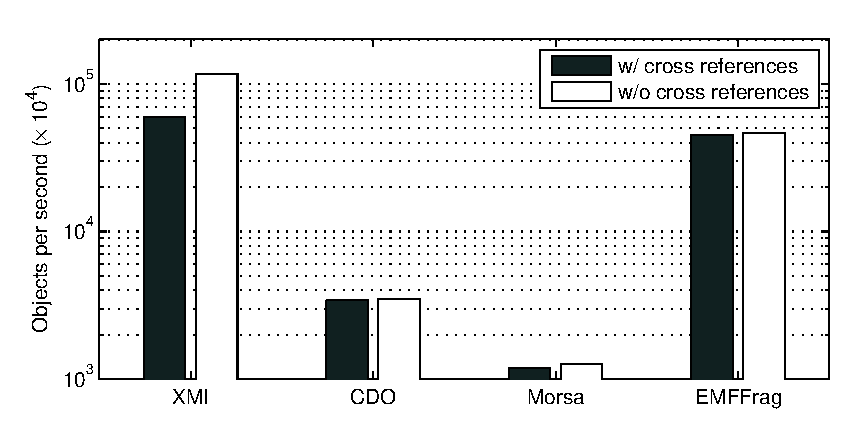
\includegraphics[width=\linewidth]{figures/createObjectsPerSecond}
\vspace{-0.26cm}
\label{fig:createObjectsPerSecond}
\caption{Number of objects per second that can be created with the different persistence frameworks.}
\end{minipage}
\hspace{0.02\linewidth}
\begin{minipage}[b]{0.48\linewidth}
\centering
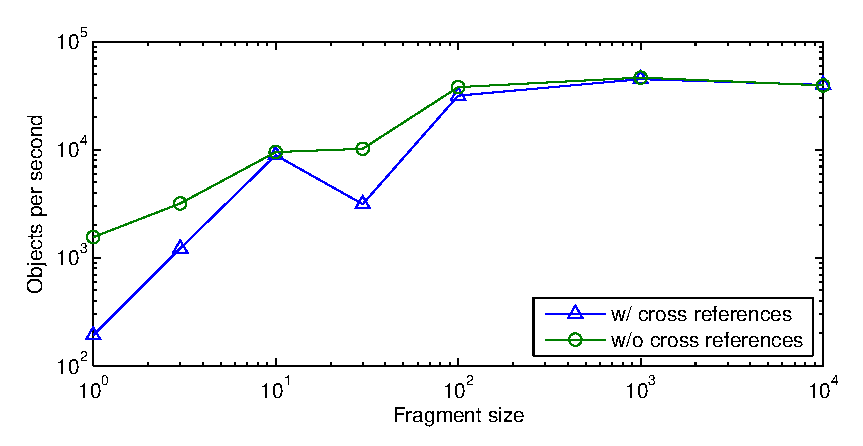
\includegraphics[width=\linewidth]{figures/createObjectsFragPerSecond}
\caption{Number of objects per second that can be created with the EMFFrag and different fragmentation granularity.}
\label{fig:createObjectsFragPerSecond}
\end{minipage}
%\vspace{0.02\linewidth}
\begin{minipage}[b]{0.48\linewidth}
\centering
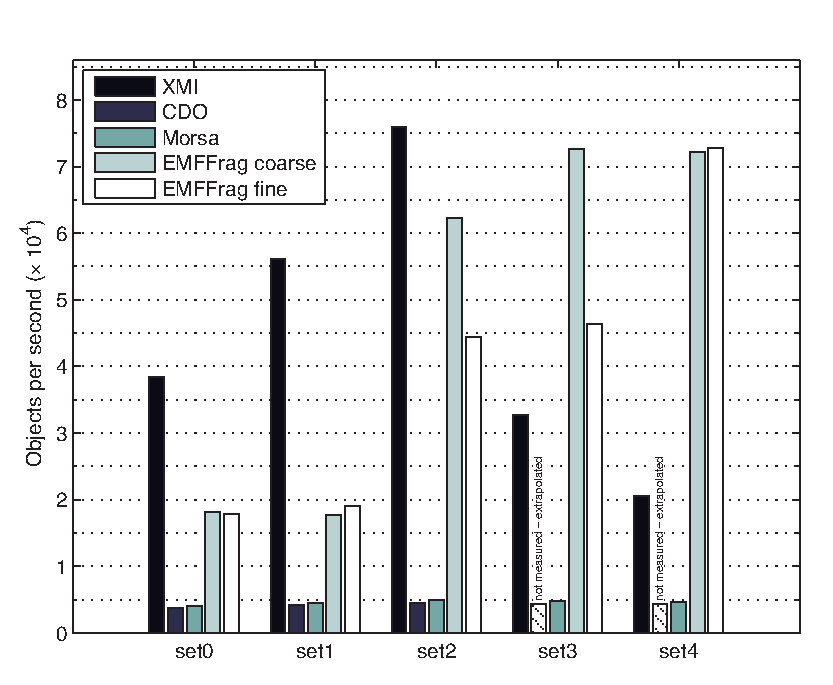
\includegraphics[width=\linewidth]{figures/grabatsTraverseObjectsPerSecondExtra}
\caption{Number of objects traversed per second during traversing the different Grabats models.}
\label{fig:grabatsTraverseTime}
\end{minipage}
\hspace{0.02\linewidth}
\begin{minipage}[b]{0.48\linewidth}
\centering
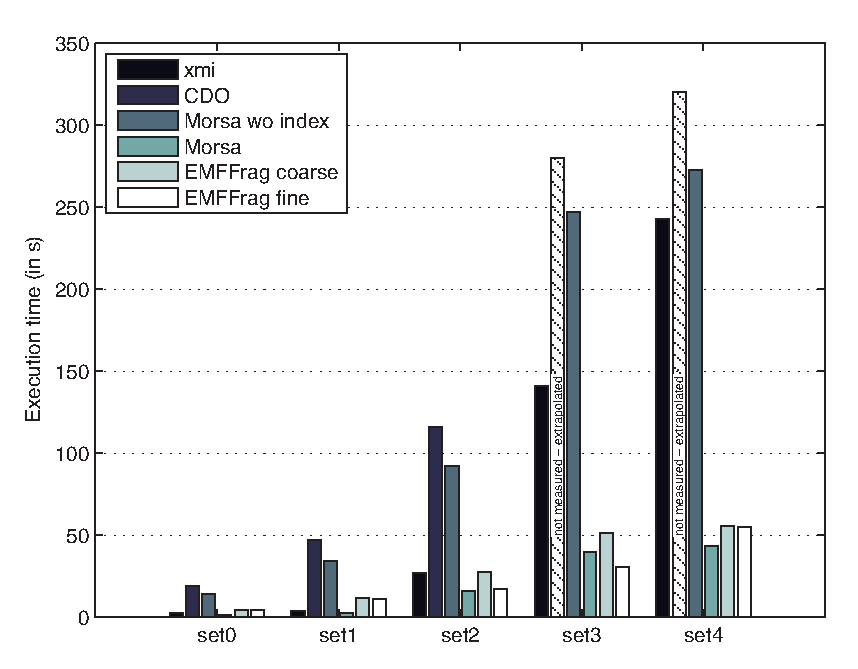
\includegraphics[width=\linewidth]{figures/grabatsQueryTimeExtra}
\caption{Execution time for querying the different Grabats models with the example query.}
\label{fig:grabatsQueryTime}
\end{minipage}
%\end{figure}
%\begin{figure}[ht]
\begin{minipage}[b]{0.48\linewidth}
\centering
%\vspace{0.04\linewidth}
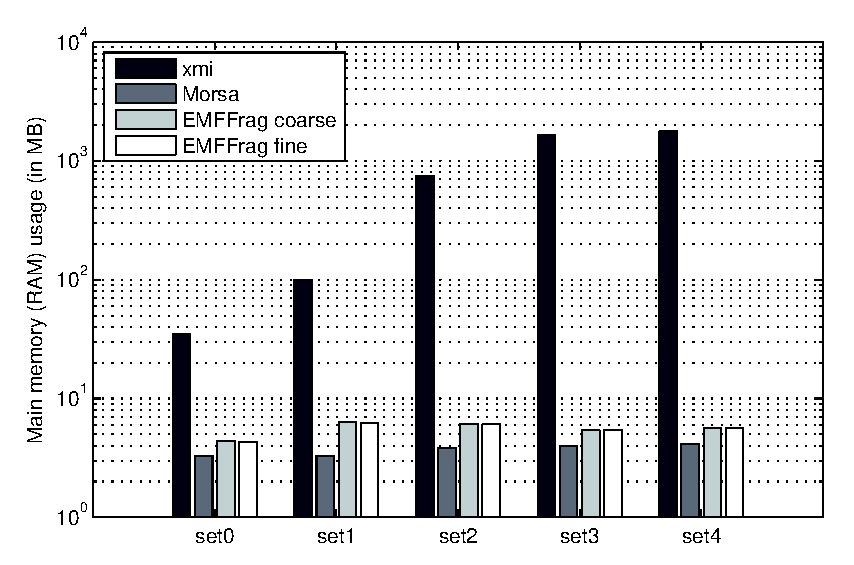
\includegraphics[width=\linewidth]{figures/grabatsTraverseMem}
\caption{Memory usage during traversal of the different Grabats models.}
\label{fig:grabatsTraverseMem}
\end{minipage}
\hspace{0.02\linewidth}
\begin{minipage}[b]{0.48\linewidth}
\centering
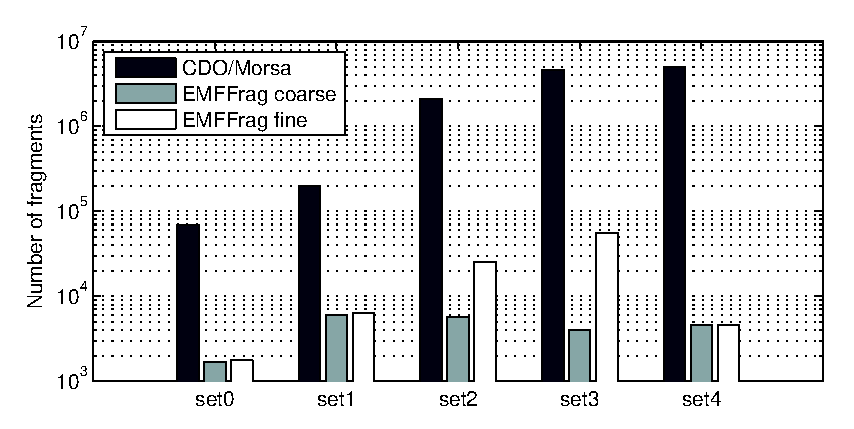
\includegraphics[width=\linewidth]{figures/grabatsFragments}
\caption{Number of fragments used by the different persistence frameworks.}
\label{fig:grabatsFragments}
\end{minipage}
\end{figure}

\tinyparagraph{Create/modify} We measured the performance of instantiating and persisting objects. A meta-model with only one class was used. We created test models with $10^5$ objects, a binary containment hierarchy, and two different densities of cross references: one cross reference per object and no cross references. We used a transaction size of $10^3$ objects for CDO and a fragment size of $10^3$ for EMFFrag.

Fig.~\ref{fig:createObjectsPerSecond} shows the average number of objects that could be persisted within one second. The number of cross-references has only a minor influence on the performance of CDO, Morsa, and EMFFrag. EMFFrag is a little slower than XMI depending on the fragment size (Fig.~\ref{fig:createObjectsFragPerSecond}). CDO and Morsa (both based on complex indices that have to be maintained) can only create less than one tenth of the objects per seconds that could be created with XMI and EMFFrag. Fig.~\ref{fig:createObjectsFragPerSecond} shows EMFFrag's create performance for different fragment sizes.

\tinyparagraph{Traverse} Fig.~\ref{fig:grabatsTraverseTime} shows the measurement results in traversed objects per second. XMI performs well for small models, but numbers deteriorate for large models. Interestingly, Morsa and CDO both use \emph{total fragmentation} and achieve both a comparable low ~4,500 objects per second. EMFFrag performs depending on the number of fragments: the less fragments the better. With the Grabats models, fragmentation allows to traverse about 10-18 times the number of objects per second than with CDO or Morsa do.

\tinyparagraph{Query} The Grabats contest also provides an example query: find all Java type declarations that contain a static method which has its containing type as return type. Depending on the persistence framework, queries can be implemented in different ways. With XMI and EMFFrag there are no indices that would help to implement the query and we have to traverse the model until we found all type declarations. CDO allows to use SQL to query and Morsa provides a meta-model class to objects index. We measured both: executing the queries with these specific query mechanisms and with the previously mentioned traverse based implementation.

The results are shown in Fig.~\ref{fig:grabatsQueryTime}. XMI performs badly for large models. CDO and Morsa with SQL and meta-class index perform best. But even though EMFFrag needs to traverse the model its performance is similar to CDO and Morsa. For \emph{set3} and fine fragmentation, EMFFrag even outperforms Morsa's index. Remember, with the fine fragmentation, EMFFrag does not need to load any method bodies to execute the query (partial load). Using the traverse implementation, CDO's and Morsa's performance difference to EMFFrag is similar to the measures for model traverse (here we basically perform a partial traverse).  

\tinyparagraph{Memory usage} During model traverse, we also measured the memory usage (Fig.~\ref{fig:grabatsTraverseMem}). XMI's memory usage is proportional to model size, because it needs to load the full models into memory. All other approaches need a comparable constant quantity of memory independent of model size.

\subsection{The Influence of Fragmentation on Partial Load Performance}

In section~\ref{sec:gains}, we looked at fragmentation analytically and provided a plot (Fig.~\ref{fig:theoryTimesSmall}) that describes the expected influence of fragmentation granularity on partial load execution times. Here, we create the same plot, but based on data measured with EMFFrag. For this purpose, we used the same simple meta-model as before (to measure create/modify) and generated models of size $10^6$ with different fragment sizes $f$. We measured the execution times for loading parts of different sizes $l$. The results are presented in Fig.~\ref{fig:measureTimeExtra}.

\begin{figure}[b]
\begin{minipage}[b]{0.48\linewidth}
\centering
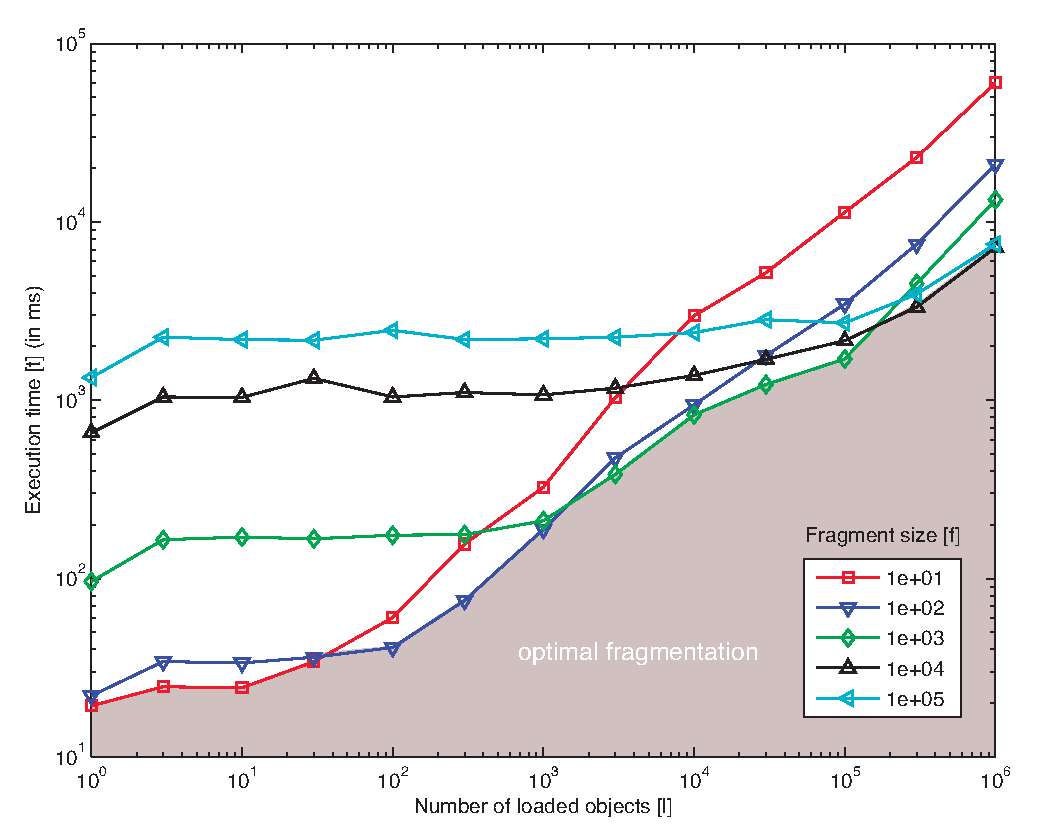
\includegraphics[width=\linewidth]{figures/measureTimesExtra}
\end{minipage}
\hspace{0.02\linewidth}
\begin{minipage}[b]{0.48\linewidth}
\centering
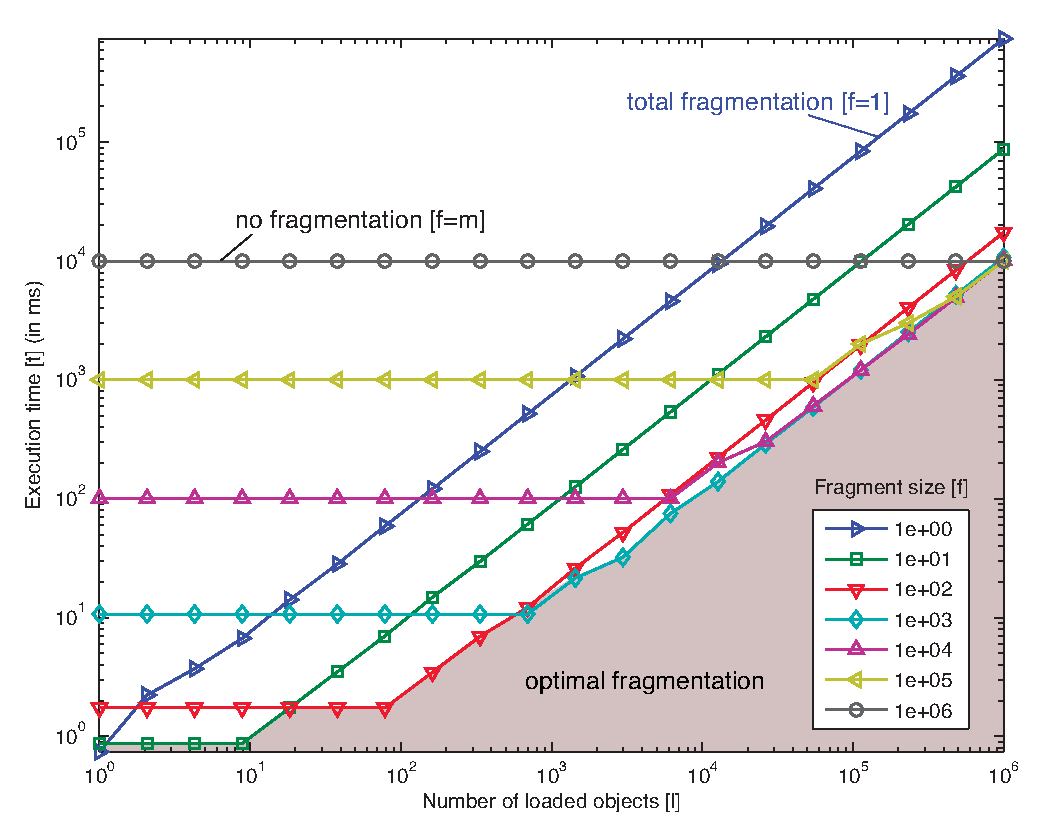
\includegraphics[width=\linewidth]{figures/theoryTimesSmallWO}
\end{minipage}
\caption{Execution times for loading model parts with different fragmentation granularity.}
\label{fig:measureTimeExtra}
\end{figure}
%
%\begin{figure}
%  \centering
%  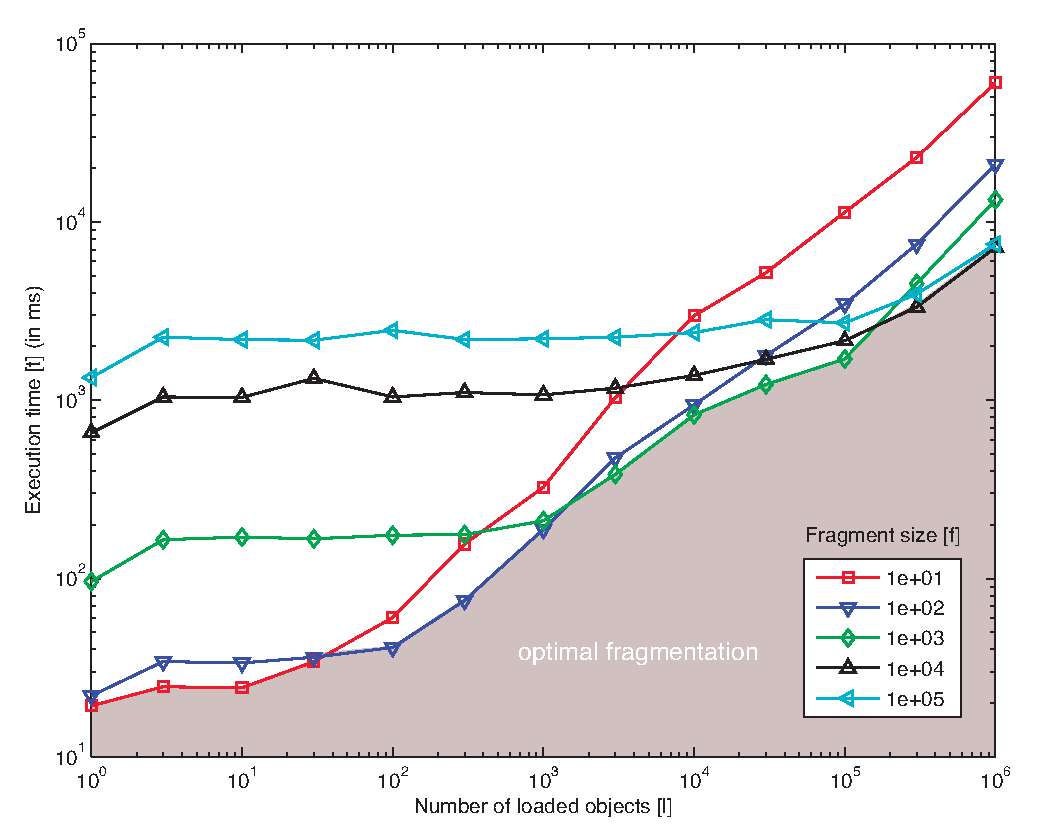
\includegraphics[width=0.65\linewidth]{figures/measureTimesExtra}
%  \caption{Execution times for loading model parts with different fragmentation granularity.}
%  \label{fig:measureTimeExtra}
%\end{figure}

The plots show a similar picture with comparable values. Although, the measured times are generally larger due to additional EMFFrag implementation overhead that was not considered in our theoretical examination.